%%%
%
% $Autor: Jana Meenakshi $
% $Datum: 2021-05-14 $
% $Pfad: PythonPackages/Contents/General/Logging $
% $Dateiname: 
% $Version: 4620 $
%
% !TeX spellcheck = en_GB/de_DE
% !TeX program = pdflatex
% !TeX encoding = utf8
% !TeX root = filename
% !TeX TXS-program:bibliography = txs:///biber
%%%



\chapter{Package \PYTHON{logging}}

\section{Introduction}

The Python logging module provides a flexible framework for emitting log messages
from Python programs. It is a part of Python’s standard library and
offers a standardized way to track events that happen when software runs. The
logging module was added to Python 2.3 and has been maintained as a key
component of Python’s standard library ever since.
This package is particularly useful for: - Debugging applications during development
- Monitoring applications in production - Tracking user activities and
system behavior - Recording error conditions and warnings - Generating audit
trails\cite{Python:2024Logging}

\begin{center}
	\includegraphics[width=0.9\textwidth]{Images/Logging/Logging_Types.png}
	\captionof{figure}{Logging\_Types.png} 
	\end{center}

\begin{itemize}
	\item Program execution flow.
	\item Errors and warnings.
	\item Information about critical events.
\end{itemize}
Instead of using print() for debugging, logging allows structured and configurable logging, making it ideal for both small scripts and large applications.
\bigskip


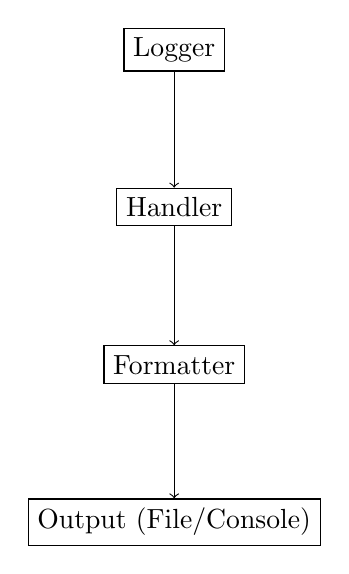
\begin{tikzpicture}[node distance=2cm]
	\node (logger) [draw] {Logger};
	\node (handler) [draw, below of=logger] {Handler};
	\node (formatter) [draw, below of=handler] {Formatter};
	\node (output) [draw, below of=formatter] {Output (File/Console)};
	
	\draw[->] (logger) -- (handler);
	\draw[->] (handler) -- (formatter);
	\draw[->] (formatter) -- (output);
\end{tikzpicture}

\section{Description}

The logging module defines a standard way to emit log messages from Python
programs. It provides a robust and highly customization logging system that can
be configured to:\cite{Python:2024Logging}

\begin{enumerate}
	\item Send output to different destinations (console, files, network sockets, etc.)
	\item Format messages in different ways
	\item Filter messages based on their severity level
	\item Handle messages from multiple modules and processes
\end{enumerate}


\subsection{Main components}
\begin{enumerate}
	\item Loggers: Entry point for logging messages.
	\item Handlers: Define where logs go (console, files, etc.).
	\item Formatters: Define how log messages are displayed.
	\item Levels: Define the severity of the logs (e.g., DEBUG, INFO, WARNING, ERROR, CRITICAL).
\end{enumerate}

\section{Installation}

The logging module is part of the Python standard library, so there is no need to install it separately. It comes pre-installed with Python.\cite{python_packages}

Steps to Verify If logging is Installed
\begin{enumerate}
	\item Open your terminal or command prompt.
	\item Check your Python version to confirm Python is installed:
	\begin{lstlisting}
	python3 --version
	\end{lstlisting}
	\item To verify the \textbf{logging} module is available, you can run a quick Python test:
	\begin{lstlisting}
		python -c "import logging; print('Logging is available and working')"
	\end{lstlisting}
	\item Expected Output:
	\begin{lstlisting}
		Logging is available and working
	\end{lstlisting}
\end{enumerate}

\SHELL{pip packageExample}

\subsection{Basic Example}

Simple Logging to Console import logging

BasicExample

\lstinputlisting[language=Python]{../Code/General/logging/BasicExample.py}	


\subsection{Logging to a File}

\lstinputlisting[language=Python]{../Code/General/logging/WritingToFile.py}	


\subsection{Using Multiple Handlers}


%\lstinputlisting[language=Python]{../Code/General/logging/MultipleHandlers.py}	



\section{Example -Description}
The logging module in Python is a powerful tool used to track events that occur while a program runs. It provides a way to log messages for debugging, monitoring, and auditing applications. Logging helps developers identify issues, track the flow of execution, and store logs for later analysis.

Key Features of Logging:
\begin{enumerate}
  \item Hierarchical Loggers – Log messages are categorized using loggers.
  \item Multiple Handlers – Allows logging to different outputs like files, console, or external systems.
  \item Configurable Log Levels – Supports different levels (DEBUG, INFO, WARNING, ERROR, CRITICAL).
  \item Custom Formatting – Messages can be formatted for readability.
  Logging is commonly used in web applications, security monitoring, and large-scale software systems.
\end{enumerate}


\section{Architecture of the Python Logging Package}


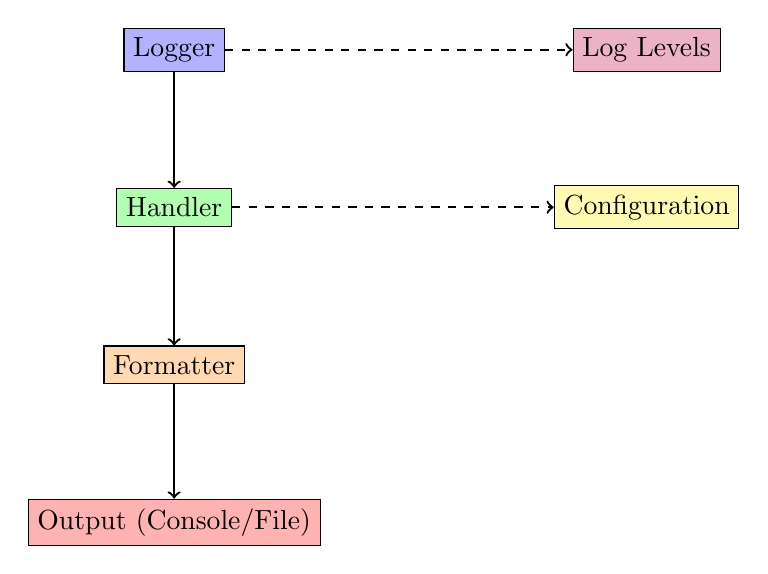
\begin{tikzpicture}[
  node distance=2cm,
  logger/.style={draw, fill=blue!30, text centered},
  handler/.style={draw, fill=green!30, text centered},
  formatter/.style={draw, fill=orange!30, text centered},
  output/.style={draw, fill=red!30, text centered},
  log_levels/.style={draw, fill=purple!30, text centered},
  config/.style={draw, fill=yellow!30, text centered}
  ]
  
  % Nodes
  \node (logger) [logger] {Logger};
  \node (handler) [handler, below of=logger] {Handler};
  \node (formatter) [formatter, below of=handler] {Formatter};
  \node (output) [output, below of=formatter] {Output (Console/File)};
  \node (log_levels) [log_levels, right of=logger, xshift=4cm] {Log Levels};
  \node (config) [config, right of=handler, xshift=4cm] {Configuration};
  
  % Connections
  \draw[->, thick] (logger) -- (handler);
  \draw[->, thick] (handler) -- (formatter);
  \draw[->, thick] (formatter) -- (output);
  \draw[->, thick, dashed] (logger) -- (log_levels);
  \draw[->, thick, dashed] (handler) -- (config);
  
\end{tikzpicture}


\subsection{Logger}

Description: The Logger is the entry point for logging messages in an application. It allows you to record events and set the severity level (e.g., DEBUG, INFO, WARNING, ERROR, CRITICAL). \cite{PythonHandler:2024}

\subsection{Code}

  \begin{lstlisting}
import logging
    
logger = logging.getLogger('my_logger')
logger.setLevel(logging.DEBUG)
logger.info('This is an info message.')
  \end{lstlisting}
  
\subsection{Usage}

 Loggers are created using logging.getLogger(name). The root logger is created by default when the logging package is imported.

  
\subsection{Handler}

  \begin{enumerate}
    \item Description: Handlers send the log messages to their final destination, which can be a console, file, or other output streams. Common handlers include \textbf{StreamHandler} and \textbf{FileHandler}.
    \item Usage: Handlers are added to loggers using the addHandler() method\cite{logging_security}
  \end{enumerate}

\subsection{Formatter}

  \begin{enumerate}
    \item   Description: Formatters specify the layout of log messages. You can define how messages appear in the log files or console, including timestamps and severity levels.
    \item Usage: Formatters are created using logging.Formatter(format\_string), and they are set for handlers using the setFormatter() method.
  \end{enumerate}
  
\subsection{Log Levels}

  \begin{enumerate}
    \item Description: Log levels indicate the severity of events. They range from DEBUG (lowest) to CRITICAL (highest). You can filter messages based on these levels.
    
    \item Usage: Set the log level using logger.setLevel(level) to control which messages get logged.\cite{logging_configuration}
  \end{enumerate}
  
\subsection{Configuration}

  \begin{enumerate}
    \item Description: Configuration of the logging system can be done through code or configuration files. This allows you to define loggers, handlers, and formatters in a structured manner.
    \item Usage: Configuration can be loaded using logging.config.fileConfig() or logging.config.dictConfig() for dictionary-based configurations.
  \end{enumerate}

\section{Example - Manual}
The manual section provides step-by-step instructions on setting up and using the logging package.

\begin{enumerate}
	\item Installing Logging Package (For Python) The logging module is included in the Python standard library, so no installation is required. However, for advanced logging features, additional packages like loguru can be installed:
	\begin{lstlisting}[style=bashstyle]
	pip install loguru
	\end{lstlisting}
	\item Basic Configuration of Logging To configure logging in Python, use the basicConfig method:
		\begin{lstlisting}[style=pythonstyle]
	import logging
	
	logging.basicConfig(level=logging.INFO,
	format='%(asctime)s - %(levelname)s - %(message)s')
	
	logger = logging.getLogger(__name__)
	logger.info("Logging is now set up!")
	\end{lstlisting}
	\bigskip
		\begin{lstlisting}[style=bashstyle]
		2025-01-31 12:00:00 - INFO - Logging is now set up!
	\end{lstlisting}
	\item Writing Logs to a File:
		\begin{lstlisting}[style=pythonstyle]
		logging.basicConfig(filename='app.log', level=logging.DEBUG,
		format='%(asctime)s - %(name)s - %(levelname)s - %(message)s')
		
		logger.debug("This is a debug message")
		logger.error("This is an error message")
	\end{lstlisting}
\end{enumerate}

\subsection{Basic Window Creation with Logging}

\begin{itemize}
	\item Importing Required Libraries:
	\begin{enumerate}
		\item \textbf{tkinter}: For creating the GUI window.
		\item \textbf{logging}: For implementing the logging mechanism.
	\end{enumerate}
	
	\item Code:
	
	\begin{lstlisting}
		import tkinter as tk
		import logging
		
		# Set up logging
		logging.basicConfig(level=logging.DEBUG, format='%(asctime)s - %(levelname)s - %(message)s')
		logger = logging.getLogger('simple_logger')
		
		def on_button_click():
		logger.info("Button clicked!")
		label.config(text="Button was clicked!")
		
		# Create the main window
		root = tk.Tk()
		root.title("Simple Logging Example")
		
		# Create a label and a button
		label = tk.Label(root, text="Press the button")
		label.pack(pady=20)
		
		button = tk.Button(root, text="Click Me", command=on_button_click)
		button.pack(pady=10)
		
		# Start the GUI event loop
		root.mainloop()
	\end{lstlisting}
	
	
	
\item Output for Logging Flow
	
	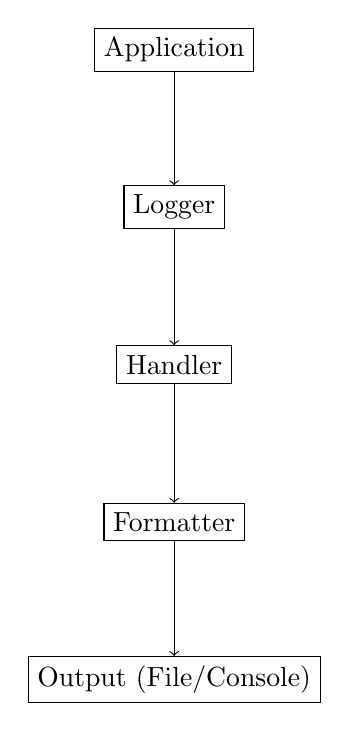
\begin{tikzpicture}[node distance=2cm]
		\node (app) [draw] {Application};
		\node (logger) [draw, below of=app] {Logger};
		\node (handler) [draw, below of=logger] {Handler};
		\node (formatter) [draw, below of=handler] {Formatter};
		\node (output) [draw, below of=formatter] {Output (File/Console)};
		
		\draw[->] (app) -- (logger);
		\draw[->] (logger) -- (handler);
		\draw[->] (handler) -- (formatter);
		\draw[->] (formatter) -- (output);
	\end{tikzpicture}
	
\end{itemize}

\section{Advanced Examples}
\subsubsection{Custom Formatter}

\begin{lstlisting}[style=pythonstyle]
	\item import logging
	import time
	class CustomFormatter(logging.Formatter):
	def formatTime(self, record, datefmt=None): ct = self.converter(record.created)
	if datefmt:
	s = time.strftime(datefmt, ct)
	else:
	t = time.strftime("%Y-%m-%d %H:%M:%S", ct) s = "%s.%03d" % (t, record.msecs)
	return s
	
	# Create logger
	logger = logging.getLogger('CustomLogger') logger.setLevel(logging.DEBUG)
	# Create handler
	handler = logging.StreamHandler() handler.setLevel(logging.DEBUG)
	# Create custom formatter
	formatter = CustomFormatter('%(asctime)s - %(name)s - %(levelname)s - %(message)s') handler.setFormatter(formatter)
	# Add handler to logger
	logger.addHandler(handler)
	# Log message
	logger.info('Test message with custom formatter')
\end{lstlisting}

\subsubsection{Rotating File Handler}

\begin{lstlisting}[style=pythonstyle]
	import logging
	from logging.handlers import RotatingFileHandler
	# Create logger
	logger = logging.getLogger('RotatingLogger') logger.setLevel(logging.INFO)
	# Create rotating file handler
	handler = RotatingFileHandler('rotating.log', maxBytes=1000, backupCount=5) handler.setLevel(logging.INFO)
	# Create formatter
	formatter = logging.Formatter('%(asctime)s - %(name)s - %(levelname)s - %(message)s') handler.setFormatter(formatter)
	# Add handler to logger
	logger.addHandler(handler)
	# Log messages
	for i in range(100): logger.info(f'Log message {i}')
\end{lstlisting}

\subsubsection{Timed Rotating File Handler}

\begin{lstlisting}[style=pythonstyle]
	import logging
	from logging.handlers import TimedRotatingFileHandler
	# Create logger
	logger = logging.getLogger('TimedRotatingLogger') logger.setLevel(logging.INFO)
	# Create timed rotating file handler
	handler = TimedRotatingFileHandler('timed_rotating.log', when='midnight', interval=1) handler.setLevel(logging.INFO)
	# Create formatter
	formatter = logging.Formatter('%(asctime)s - %(name)s - %(levelname)s - %(message)s') handler.setFormatter(formatter)
	# Add handler to logger
	logger.addHandler(handler)
	# Log message
	logger.info('This log will rotate at midnight')
\end{lstlisting}

\section{Configuration Examples}
\subsection{Dictionary Configuration}


\begin{lstlisting}[style=pythonstyle]
import logging.config
config = {
	'version': 1, 'formatters': {
		'detailed': {
			'class':  'logging.Formatter',
			'format': '%(asctime)s - %(name)s - %(levelname)s - %(message)s'
		}
	},
	'handlers': {
		'console': {
			'class': 'logging.StreamHandler', 'level': 'INFO',
			'formatter': 'detailed'
		},
		'file': {
			'class': 'logging.FileHandler', 'filename': 'logging_config.log', 'level': 'DEBUG',
			
			
			
			'formatter': 'detailed'
		}
	},
	'loggers': {
		'myapp': {
			'handlers': ['console', 'file'], 'level': 'DEBUG',
			'propagate': False
		}
	}
}
logging.config.dictConfig(config) logger = logging.getLogger('myapp') logger.info('Application started')

\end{lstlisting}

\subsubsection{JSON Configuration}
\begin{lstlisting}[style=pythonstyle]
	import json
	import logging.config
	config = {
		"version": 1, "disable_existing_loggers": False, "formatters": {
			"simple": {
				"format": "%(asctime)s - %(name)s - %(levelname)s - %(message)s"
			}
		},
		"handlers": {
			"console": {
				"class": "logging.StreamHandler", "level": "DEBUG",
				"formatter": "simple", "stream": "ext://sys.stdout"
			},
			"file": {
				"class": "logging.FileHandler", "level": "INFO",
				"formatter": "simple", "filename": "app.log",
				"mode": "w"
			}
		},
		"loggers": {
			"": {
				
				
				
				"level": "INFO",
				"handlers": ["console", "file"], "propagate": True
			}
		}
	}
	with open('logging_config.json', 'w') as f: json.dump(config, f, indent=4)
	logging.config.fileConfig('logging_config.json')  logger = logging.getLogger( name )
\end{lstlisting}

\section{Exception Handling Examples}
\subsection{Basic Exception Logging}
\begin{lstlisting}[style=pythonstyle]
	import logging
	logger = logging.getLogger( name ) logger.setLevel(logging.INFO)
	handler = logging.StreamHandler()
	formatter = logging.Formatter('%(asctime)s - %(name)s - %(levelname)s - %(message)s') handler.setFormatter(formatter)
	logger.addHandler(handler)
	def divide(x, y):
	try:
	result = x / y
	logger.info(f'Division result: {result}')
	return result
	except ZeroDivisionError:
	logger.error('Division by zero!', exc_info=True)
	raise
	except Exception as e:
	logger.error(f'Unexpected error: {str(e)}', exc_info=True)
	raise
	
	# Test the function
	try:
	divide(10, 0)
	except:
	pass
\end{lstlisting}

\subsection{Contextual Exception Logging}
\begin{lstlisting}[style=pythonstyle]
	import logging
	import traceback
	from contextlib import contextmanager
	logger = logging.getLogger( name ) logger.setLevel(logging.INFO)
	handler = logging.StreamHandler()
	formatter = logging.Formatter('%(asctime)s - %(name)s - %(levelname)s - %(message)s') handler.setFormatter(formatter)
	logger.addHandler(handler)
	@contextmanager
	def log_errors(operation):
	try:
	yield
	except Exception as e:
	logger.error(f'Error during {operation}: {str(e)}') logger.debug(f'Traceback: {traceback.format_exc()}') raise
	
	def process_data(data):
	with log_errors('data processing'):
	if not data:
	raise ValueError('Empty data')
	return data.upper()
	# Test the function
	try:
	process_data(None)
	except:
	pass
\end{lstlisting}

\section{Advanced Features}
\subsection{Custom Log Levels}
\begin{lstlisting}[style=pythonstyle]
	import logging
	# Define custom log levels
	VERBOSE = 15
	TRACE = 5
	# Add custom level names
	logging.addLevelName(VERBOSE,  'VERBOSE')
	
	
	
	logging.addLevelName(TRACE,  'TRACE')
	# Create custom logging methods
	def verbose(self, message, *args, **kwargs):
	if self.isEnabledFor(VERBOSE): self._log(VERBOSE, message, args, **kwargs)
	def trace(self, message, *args, **kwargs):
	if self.isEnabledFor(TRACE):
	self._log(TRACE, message, args, **kwargs)
	# Add methods to Logger class logging.Logger.verbose = verbose logging.Logger.trace = trace
	# Configure logging logging.basicConfig(level=TRACE)  logger = logging.getLogger(  name  )
	# Use custom levels logger.trace('Trace message') logger.verbose('Verbose message') logger.debug('Debug message') logger.info('Info message')
\end{lstlisting}

\subsection{Filter Implementation}
\begin{lstlisting}[style=pythonstyle]
	import logging
	class ContextFilter(logging.Filter):
	"""
	This filter adds contextual information to log records. """
	def  init (self, user): self.user = user
	def filter(self, record): record.user = self.user return True
	# Configure logging
	logger = logging.getLogger( name ) logger.setLevel(logging.INFO)
	# Create handler
	handler = logging.StreamHandler()
	
	
	
	handler.setLevel(logging.INFO)
	# Create formatter that uses the additional field
	formatter = logging.Formatter('%(asctime)s - %(user)s - %(levelname)s - %(message)s') handler.setFormatter(formatter)
	# Add filter and handler to logger logger.addFilter(ContextFilter('admin'))  logger.addHandler(handler)
	# Log messages
	logger.info('Admin action performed')
\end{lstlisting}

\subsection{Queue Handler}
\begin{lstlisting}[style=pythonstyle]
	import logging import queue import threading import time
	from logging.handlers import QueueHandler, QueueListener
	# Create queue
	log_queue = queue.Queue(-1)	# No limit on size
	
	# Configure queue handler
	queue_handler = QueueHandler(log_queue)
	# Configure logger
	logger = logging.getLogger( name ) logger.setLevel(logging.INFO) logger.addHandler(queue_handler)
	# Configure listener
	handler = logging.StreamHandler()
	handler.setFormatter(logging.Formatter('%(asctime)s - %(name)s - %(levelname)s - %(message) listener = QueueListener(log_queue, handler)
	listener.start()
	# Function that logs messages
	def worker():
	for i in range(5):
	logger.info(f'Log message {i} from worker thread') time.sleep(0.1)
	# Create and start worker thread
	thread = threading.Thread(target=worker)
	
	
	
	thread.start()
	# Main thread logs messages
	for i in range(5):
	logger.info(f'Log message {i} from main thread') time.sleep(0.1)
	# Wait for worker thread to finish
	thread.join()
	# Stop the listener
	listener.stop()
\end{lstlisting}

\section{Best Practices}
\subsection{Logging Pattern for Libraries}
\begin{lstlisting}[style=pythonstyle]
	import logging
	# Create a logger for the library
	logger = logging.getLogger(  name  )
	# Don't add any handlers
	logger.addHandler(logging.NullHandler())
	def library_function():
	"""
	Example library function that logs messages. """
	logger.debug('Entering library_function')
	try:
	# Do something
	logger.info('Operation successful')
	except Exception as e:
	logger.error('Operation failed: %s', str(e), exc_info=True)
	raise finally:
	logger.debug('Exiting library_function')
\end{lstlisting}

\section{Example - Code}
Here are different logging scenarios with Python's logging module:

\begin{enumerate}
	\item Logging to Both Console and File
	\begin{lstlisting}[style=pythonstyle]
	import logging
	
	logger = logging.getLogger('MyApp')
	logger.setLevel(logging.DEBUG)
	
	# Create handlers
	console_handler = logging.StreamHandler()
	file_handler = logging.FileHandler('app.log')
	
	# Set log levels
	console_handler.setLevel(logging.INFO)
	file_handler.setLevel(logging.DEBUG)
	
	# Define format
	formatter = logging.Formatter('%(asctime)s - %(name)s - %(levelname)s - %(message)s')
	console_handler.setFormatter(formatter)
	file_handler.setFormatter(formatter)
	
	# Add handlers
	logger.addHandler(console_handler)
	logger.addHandler(file_handler)
	
	# Logging messages
	logger.debug("Debugging info")
	logger.info("General info")
	logger.warning("This is a warning")
	logger.error("Error occurred")
	logger.critical("Critical issue!")
	\end{lstlisting}
	
\end{enumerate}

\section{Example - Files}
Logging can be stored in different file formats and locations:

\begin{enumerate}
	\item Plain Text Log Files – Default logging format:
	\begin{lstlisting}[style=pythonstyle]
		logging.basicConfig(filename='logfile.txt', level=logging.INFO)
		logging.info("Logging to a text file.")
	\end{lstlisting}
	
	\item Output
		\begin{lstlisting}[style=bashstyle]
	2025-01-31 12:00:00 - INFO - Logging to a text file.
	\end{lstlisting}
	
\end{enumerate}

\section{Further Reading}



\nocite{Abadi:2016}

	% Überschrift ein Level unter `refsection=chapter`, also \section*:
   \printbibliography[heading=subbibliography, segment=\therefsegment]










